\section{Evaluation}
We first applied our approaches to several real-world dataset and compare our method with the uniform random sampling. Then we conduct several user studies on specific analysis tasks. 
\subsection{Experimental results}
In this section, we will briefly evaluate our method by case studies. We will first make a brief comparison between the VQGTS and uniform random sampling at different granularities. Then we will show how VQGTS further improves the visual quality by taking the \QM{representative} into consideration. At last, we will extend our method to more dataset and demonstrate the effectiveness of propsoed method.
\subsubsection{VTGS and uniform random sampling}
Our first example uses taxi trajectories collected from 442 active taxis in the city of Porto, Portugal~\footnote{\url{http://www.geolink.pt/ecmlpkdd2015-challenge/dataset.html}}. Figure~\ref{fig:random_proposed} shows the comparison among the ground truth, uniform random sampling and the VQGTS. Both random sampling and VQGTS method take $0.01$ as the sampling rate. 
In the overview(map scale at 11), based on the ground truth(shown as figure~\ref{fig:random_proposed} A), the random sampling(shown as figure~\ref{fig:random_proposed} C) has a very poor the visual quality especially for the boundary region because very few trajectories are preserved by the sampling methods. That's because in the city, most of the taxi trips concentrate to the downtown, thus the sampled trajectories are more likely located in the downtown, which lead to a serious visual information loss.  
But our method(shown as figure~\ref{fig:random_proposed} B) are visually very close to the ground truth even in the margin regions. 
%In the overview, VQGTS(figure~\ref{fig:random_proposed} B) looks much more close to the ground truth(figure~\ref{fig:random_proposed} A) than the random method(figure~\ref{fig:random_proposed} C) especially for the boundary areas which . We further compare the details of region a and b. 
We further compare the visualization at the detail level(map scale at 15).
The figures in second rows depict the detail view of the ground truth, VQGTS and sampling at the region shown in Figure~\ref{fig:random_proposed} a, which is the city center of Porto. Comparing with VQGTS, random sampling preserve the general trajectory framework but miss the details(As the figure~\ref{fig:random_proposed}F, G shown). However, for the fridge of the city where the trajectories are spare distributed, the VQGTS has clear advantage than random sampling because it well preserve the detail structure of trajectories as shown in the black region in the figure~\ref{fig:random_proposed} H and I. This case demonstrates our proposed sampling method works well in both overview and detail view compared with the random sampling method.

\begin{figure}[t]
	\centering
	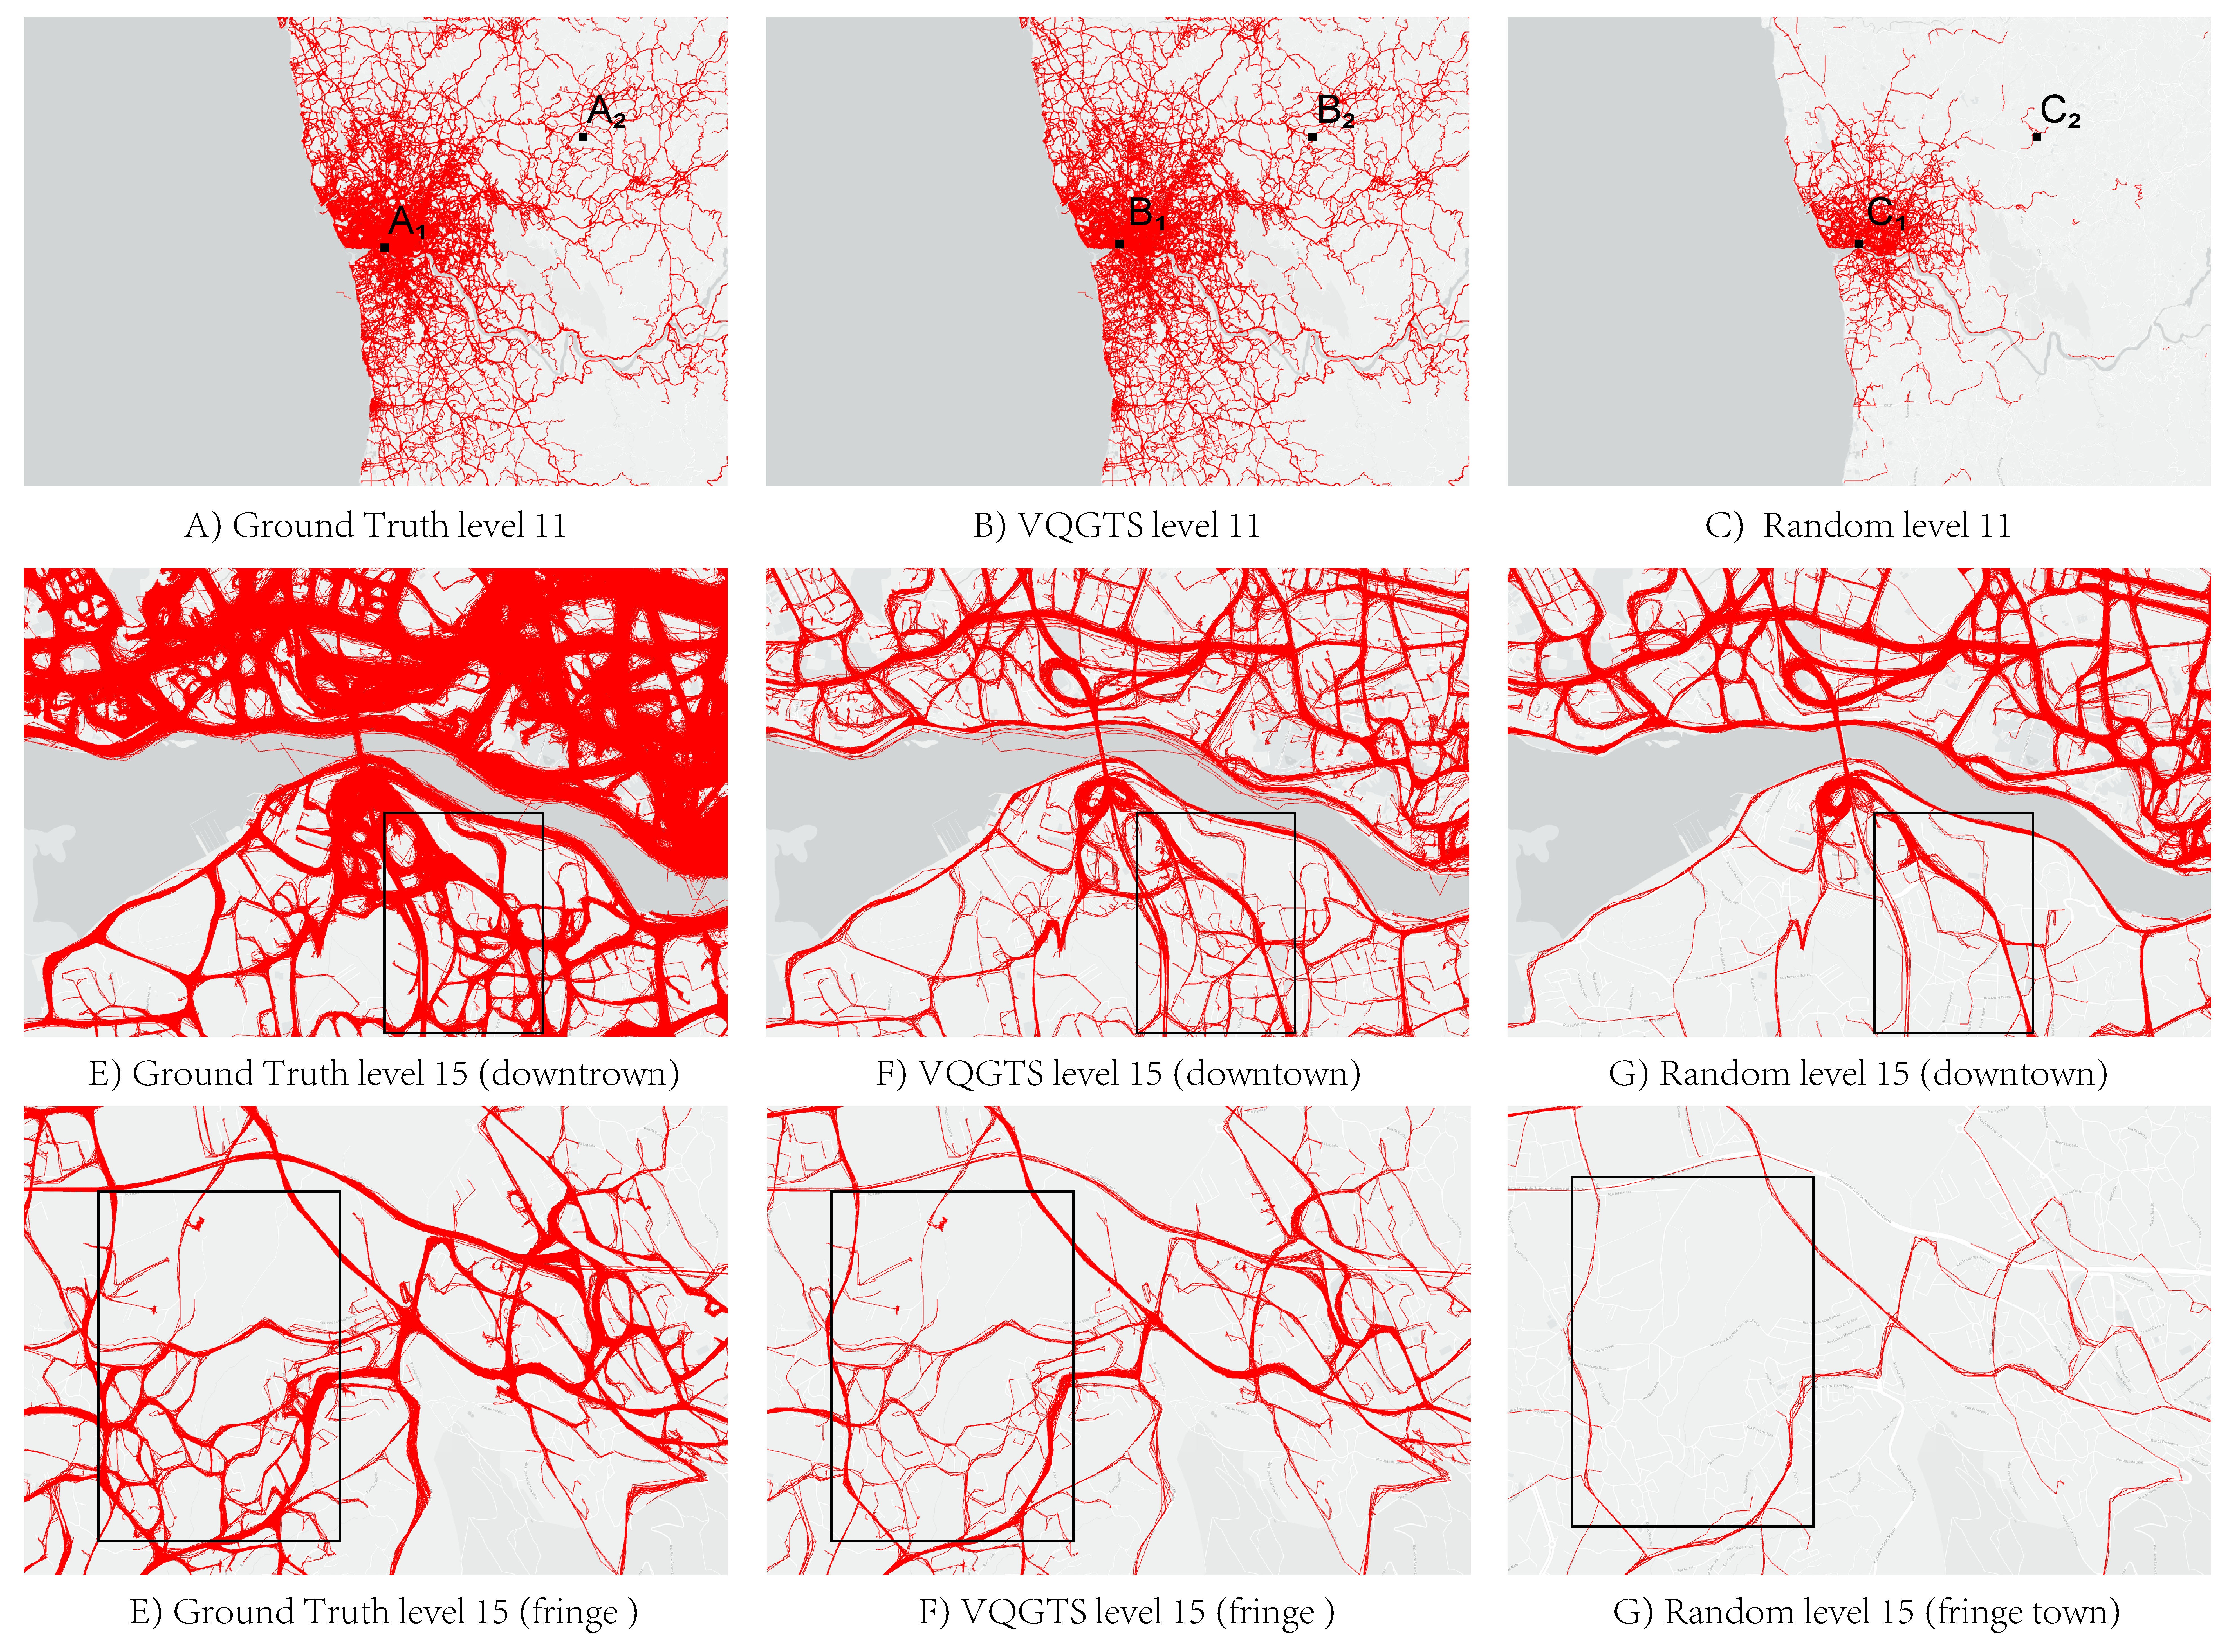
\includegraphics[width=0.48\textwidth]{pictures/experiment_study/Mehtod_resolution_study.pdf}
	\vspace{-5mm}
	\caption{Result evaluation between proposed method and uniform random sampling. The images in the three columns indicate the visualization results for full dataset, proposed method, and uniform random sampling respectively. The visualizations in the first row shows the overview. The visualizations in the second the third row indicate the detail level visualization of region 1 and region 2. }
	\vspace{-5mm}
	\label{fig:random_proposed}
\end{figure}

\subsubsection{Representativeness parameters analysis}
To analysis the parameters  $\delta$


\begin{figure}[t]
	\centering
	\vspace{2mm}
	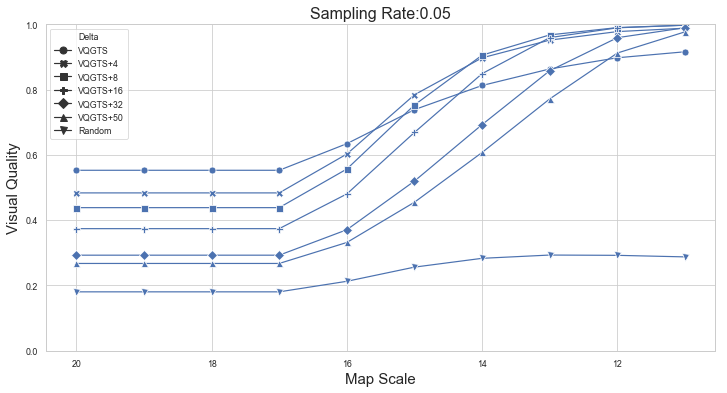
\includegraphics[width=0.48\textwidth]{pictures/experiment_study/quanlity.png}
	\caption{Visual quality chart. X axis indicates map scale from detail view to overview; y axis indicate the visual quality. }
	\vspace{0mm}
	\label{fig:quality_chart}
\end{figure}

\subsection{User study}
\setlist{nolistsep}
\begin{itemize}[noitemsep]
    \item Visual similarity
    \item Identify outliers
\end{itemize}

\subsection{Expert overview}

